%%%%%%%%%%%%%%%%%%%%%%%%%%%%%%%%%%%%%%%%%%%%%%%%%%%%%%%%%%%%%%%%%%%%%%%%%%%%%%%%%
%
% Purpose:  Verification part of V&V for the Euler model
%
% 
%
%%%%%%%%%%%%%%%%%%%%%%%%%%%%%%%%%%%%%%%%%%%%%%%%%%%%%%%%%%%%%%%%%%%%%%%%%%%%%%%%

% \section{Verification}

%%% code imported from old template structure
%\inspection{<Name of Inspection>}\label{inspect:<label>}
% <description> to satisfy  
% requirement \ref{reqt:<label>}.

 For testing the \EulerDesc\, a single vehicle was initialized in one of 3 orbits: an equatorial circular orbit, an inclined orbit, and an eccentric equatorial orbit.  An LVLH frame was also generated, and the Euler angles between the vehicle body frame (the subject frame), and the LVLH frame (the reference frame), were computed.  

\test{Verification of \EulerDesc\ Output Data}\label{test:Euler}

\begin{description}
\item{Purpose:}\newline
To demonstrate that the output from the \EulerDesc\ provides meaningful data.

\item{Requirements:}\newline
Satisfactory conclusion of this test satisfies requirement \ref{reqt:Euler}

\item{Procedure:}\newline
Two cases were considered, one in which the vehicle frame was initially aligned with the LVLH frame, and one in which it was given an initial relative attitude.  In both cases, the vehicle body frame was initialized with no rotation (with respect to the inertial frame).  Since the LVLH frame maintains an orientation dependent upon the position of the origin, the two frames rotate with respect to one another.  The angles generated by this orbital motion are considered.

\item{Predictions:}  
In the LVLH frame, the frame-to-frame relative rotation will appear as a pitch (rotation about the LVLH y-axis).  In the tests in which the two frames are initially aligned, that is equivalent to a pitch in the body frame.  Both transformations should exhibit slowly oscillating pitch values, with constant zero values for yaw and roll.

When the two frames are not initially aligned, in general, the variation of angles resulting from the varying relative attitude will be across all three axes.  Exceptions to this rule include transformations from body to LVLH that end with a pitch, or those from LVLH to body that start with a pitch.  This is due to the order of calculation, consider the transformation from body to LVLH:

The transformation from body to initial LVLH frame is constant, and the LVLH rotates with respect to the initial LVLH frame on its y-axis; a transformation from body to LVLH can be seen as a combination of transformations from body to the initial LVLH frame followed by one from the initial LVLH frame to LVLH, which comprises only a pitch component.  Therefore, if pitch is last in the order, the two pitch adjustments simply add; the roll and yaw are due to the constant difference between body and initial LVLH, and so should remain constant, whereas the pitch should start at some pre-assigned value, and exhibit the same periodic variation thereafter that was seen in the case of the initially aligned frames.  The same argument can be traced in reverse for the reverse transformation.

For other sets in which the pitch is calculated in an inconvenient sequence (second or third, or first from body frame to reference frame, or last in reference frame to body frame), the effect in the yaw and roll angles of the addition of the pitch due to the variational relative frame rotation will manifest as a time dependency on all 3 axes, due to the cross-coupling effects of rotational sequences.

The variation with time in the rate at which the angles change will be constant for the circular orbits, but variable for the elliptic orbits.

For further confirmation of the data, the euler angles of the vehicle with respect to the inertially-oriented planetary axes we investigated, these should show no variation.

\item{Results:}
All output data confirmed expectations, within numerical precision.  Some expected constant values were not quite constant, but exhibited some very small oscillatory or noisy behavior.  

For the aligned frames, the YRP, RYP, PYR, and PRY sequences showed the pitch slowly changing  from $\pm \pi$ to $\mp \pi$ before immediately resetting.  The YPR and RPY sequences had the pitch varying only between $\pm \frac{\pi}{2}$, and doing so with constant ramps up and down.  For these two sequences, the roll and pitch also switched to $\pm \pi$ during the time that the pitch was decreasing, and returned to zero while the pitch was increasing.  These solutions are completely valid, and illustrate that there is more than one way to represent a particular orientation.  These results were valid for both the LVLH-body and body-LVLH orientations. See figures~\ref{fig:euleralignedpyr} and~\ref{fig:euleralignedrpy} for Pitch-Yaw-Roll and Roll-Pitch-Yaw sequences.

\begin{figure}[!ht]
\begin{center}
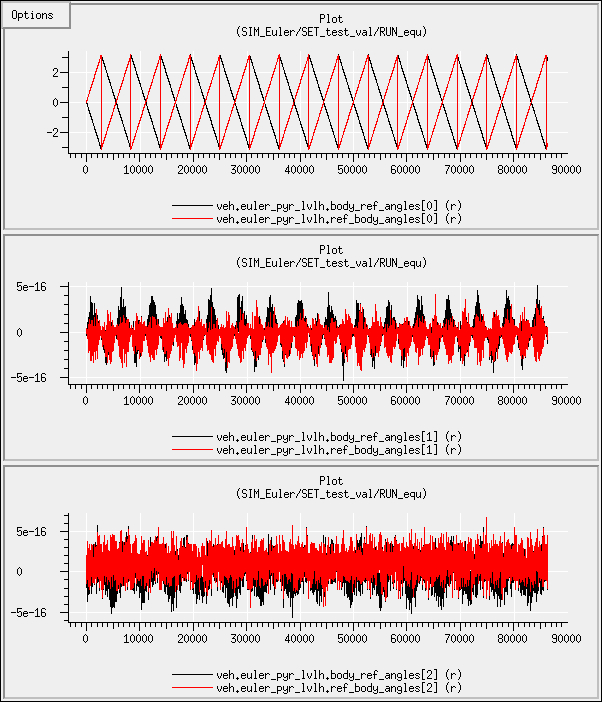
\includegraphics[width=5in]{figures/euler_aligned_pyr.jpg}
\caption{The Euler angles for the case in which the LVLH frame and body frame were initially aligned, and rotating with respect to each other on their respective pitch axes, expressed in a Pitch-Yaw-Roll sequence.}
\label{fig:euleralignedpyr}
\end{center}
\end{figure}

\begin{figure}[!ht]
\begin{center}
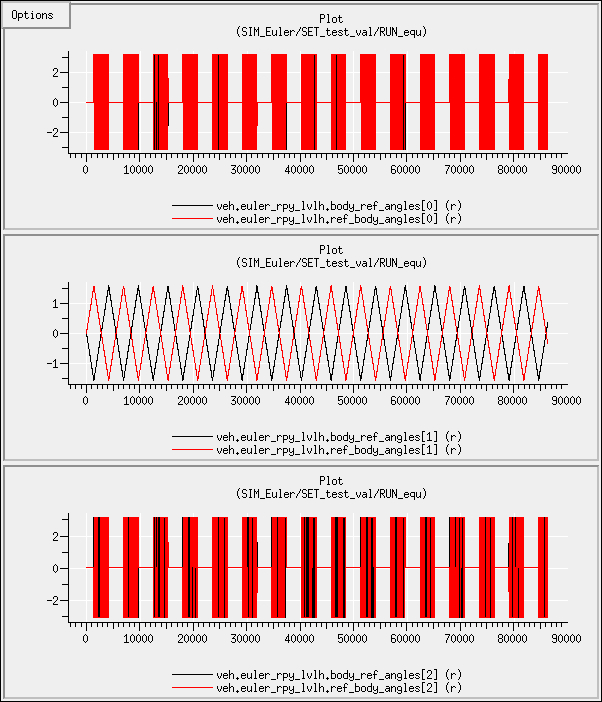
\includegraphics[width=5in]{figures/euler_aligned_rpy.jpg}
\caption{The Euler angles for the case in which the LVLH frame and body frame were initially aligned, and rotating with respect to each other on their respective pitch axes, expressed in a Roll-Pitch-Yaw sequence.  Notice that the Pitch has a total range of only $\pi$ radians; this is compensated for by the combined effect of adding in $\pi$ rotations on the yaw and roll axes.}
\label{fig:euleralignedrpy}
\end{center}
\end{figure}

For the tests in which the frames were not initially aligned, those with Pitch in the correct sequencing showed the similar pattern to the aligned frames, as expected.  Other sequences had periodic behavior.  See Figures~\ref{fig:eulernonalignedpyr},~\ref{fig:eulernonalignedrpy}, and~\ref{fig:eulernonalignedyrp} for Pitch-Yaw-Roll, Roll-Pitch-Yaw, and Yaw-Roll-Pitch sequences.

\begin{figure}[!ht]
\begin{center}
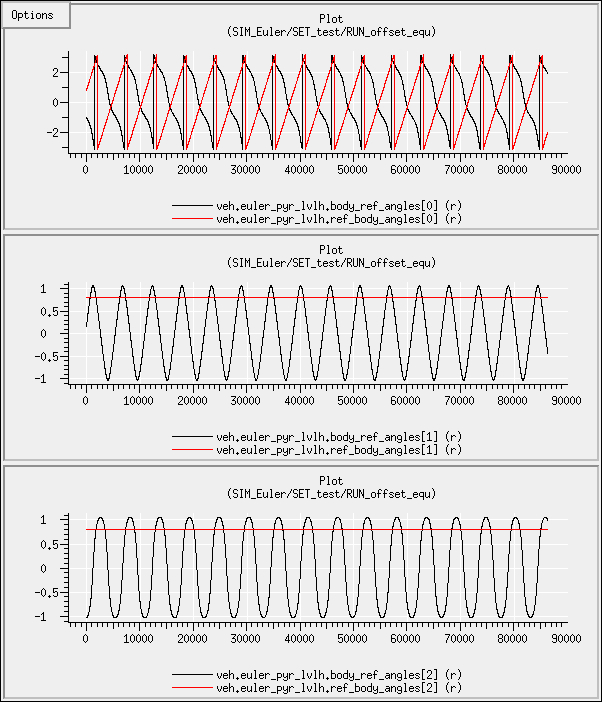
\includegraphics[width=5in]{figures/euler_nonaligned_pyr.jpg}
\caption{The Euler angles for the case in which the LVLH frame and body frame were initially un-aligned, and rotating with respect to each other on the pitch axis of the LVLH reference frame.  Angles are expressed in a Pitch-Yaw-Roll sequence.  Notice that when Pitch is first in the sequence, the angles associated with the transformation from the LVLH frame to the body frame (expressed in the LVLH frame) show a similar pattern to that in Figure~\ref{fig:euleralignedpyr}, but that is not the case when representing the relative attitude from the body frame to the LVLH frame (this is expressed in the body frame).}
\label{fig:eulernonalignedpyr}
\end{center}
\end{figure}

\begin{figure}[!ht]
\begin{center}
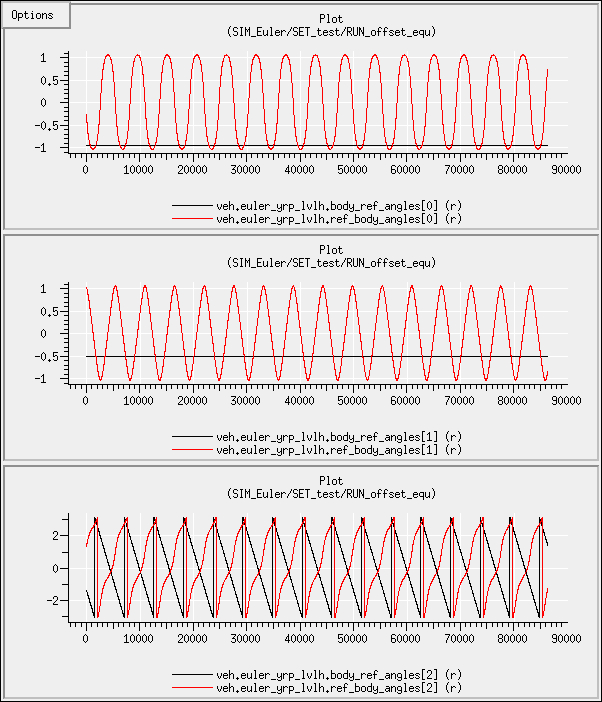
\includegraphics[width=5in]{figures/euler_nonaligned_yrp.jpg}
\caption{The Euler angles for the case in which the LVLH frame and body frame were initially un-aligned, and rotating with respect to each other on the pitch axis of the LVLH reference frame.  Angles are expressed in a Yaw-Roll-Pitch sequence.  Notice that when Pitch is last in the sequence, the angles associated with the transformation from body frame to LVLH (expressed in body frame) show a similar pattern to that in Figure~\ref{fig:euleralignedpyr}, but that is not the case when representing the relative attitude from the LVLH frame to the body frame (this is expressed in the LVLH frame).}
\label{fig:eulernonalignedyrp}
\end{center}
\end{figure}

\begin{figure}[!ht]
\begin{center}
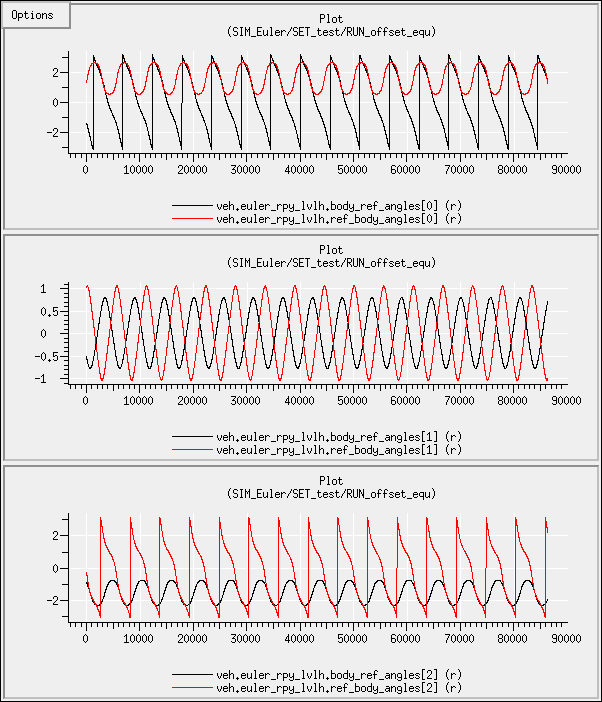
\includegraphics[width=5in]{figures/euler_nonaligned_rpy.jpg}
\caption{The Euler angles for the case in which the LVLH frame and body frame were initially un-aligned, and rotating with respect to each other on the pitch axis of the LVLH reference frame.  Notice that the variation is non-sinusoidal, and that the amplitudes differ between the two representations of the transformation.}
\label{fig:eulernonalignedrpy}
\end{center}
\end{figure}




\end{description}
